\documentclass[%
oneside,                 % oneside: electronic viewing, twoside: printing
final,                   % draft: marks overfull hboxes, figures with paths
10pt]{article}

\listfiles               %  print all files needed to compile this document

\usepackage[a4paper, total={6in, 8in}]{geometry}
\usepackage[totoc]{idxlayout}   % for index in the toc
\usepackage[nottoc]{tocbibind}  % for references/bibliography in the toc

\usepackage{relsize,makeidx,color,setspace,amsmath,amsfonts,amssymb}
\usepackage[table]{xcolor}
\usepackage{bm,ltablex,microtype}
\usepackage{comment} 
\usepackage[pdftex]{graphicx}

\usepackage{fancyvrb} % packages needed for verbatim environments

\usepackage[T1]{fontenc}
%\usepackage[latin1]{inputenc}
\usepackage{ucs}
\usepackage[utf8x]{inputenc}

\usepackage{lmodern}         % Latin Modern fonts derived from Computer Modern


\usepackage{pgfplotstable, booktabs}

\pgfplotstableset{
    every head row/.style={before row=\toprule,after row=\midrule},
    every last row/.style={after row=\bottomrule}
}





% Hyperlinks in PDF:
\definecolor{linkcolor}{rgb}{0,0,0.4}
\usepackage{hyperref}
\hypersetup{
    breaklinks=true,
    colorlinks=true,
    linkcolor=linkcolor,
    urlcolor=linkcolor,
    citecolor=black,
    filecolor=black,
    %filecolor=blue,
    pdfmenubar=true,
    pdftoolbar=true,
    bookmarksdepth=3   % Uncomment (and tweak) for PDF bookmarks with more levels than the TOC
    }
%\hyperbaseurl{}   % hyperlinks are relative to this root

\setcounter{tocdepth}{2}  % levels in table of contents

% --- fancyhdr package for fancy headers ---
\usepackage{fancyhdr}
\fancyhf{} % sets both header and footer to nothing
\renewcommand{\headrulewidth}{0pt}
\fancyfoot[LE,RO]{\thepage}
% Ensure copyright on titlepage (article style) and chapter pages (book style)
\fancypagestyle{plain}{
  \fancyhf{}
  \fancyfoot[C]{{\footnotesize \copyright\ 1999-2018, "Computational Physics I FYS3150/FYS4150":"http://www.uio.no/studier/emner/matnat/fys/FYS3150/index-eng.html". Released under CC Attribution-NonCommercial 4.0 license}}
%  \renewcommand{\footrulewidth}{0mm}
  \renewcommand{\headrulewidth}{0mm}
}
% Ensure copyright on titlepages with \thispagestyle{empty}
\fancypagestyle{empty}{
  \fancyhf{}
  \fancyfoot[C]{{ }}
  \renewcommand{\footrulewidth}{0mm}
  \renewcommand{\headrulewidth}{0mm}
}

\pagestyle{fancy}


% prevent orhpans and widows
\clubpenalty = 10000
\widowpenalty = 10000

% --- end of standard preamble for documents ---


% insert custom LaTeX commands...

\raggedbottom
\makeindex
\usepackage[totoc]{idxlayout}   % for index in the toc
\usepackage[nottoc]{tocbibind}  % for references/bibliography in the toc
\usepackage{listings}
\usepackage[normalem]{ulem} 	%for tables
\useunder{\uline}{\ul}{}
\usepackage{hyperref}
\usepackage[section]{placeins} %force figs in section

\usepackage{natbib}

\usepackage[toc,page]{appendix} % appenix


%-------------------- end preamble ----------------------

\begin{document}

% matching end for #ifdef PREAMBLE

\newcommand{\exercisesection}[1]{\subsection*{#1}}


% ------------------- main content ----------------------



% ----------------- title -------------------------

\thispagestyle{empty}

\begin{center}
{\LARGE\bf
\begin{spacing}{1.25}
Regression analysis and re-sampling methods
\end{spacing}
}
\end{center}

% ----------------- author(s) -------------------------

\begin{center}
{\bf Johan Nereng}
\end{center}

    \begin{center}
% List of all institutions:
\centerline{{\small Department of Physics, University of Oslo, Norway}}
\end{center}
    
% ----------------- end author(s) -------------------------

% --- begin date ---
\begin{center}
Sep 30, 2019
\end{center}
% --- end date ---

\vspace{5cm}
\begin{abstract}

\end{abstract}

\newpage

\section{Introduction}
The main aim of this project is to study in more detail various regression methods,
including the Ordinary Least Squares (OLS) method, Ridge regression and finally
Lasso regression, including use of resampling. Start by fitting polynomials to Franke's function (see Methods). 

Having established the model and method, the models are further evaluated using resamling
techniques such as cross-validation.


choice of modelling based on insight. Terrain possbily polynomial ? use franke function to test algorithms. 

Linear regression models the relationship between the response or target and the predictors linearly. In this project, three different methods are applied to fit the model to the data. Ordinary Least Squares (OLS), Ridge, and Lasso. Since this project assumes that the 

 Trying to find the relationship between an independent and dependent variables chose approximation ,a..a.s

it is normal to use y for predictors in litteratur,and x0 x1 etc. but for shorthand purposes, x1x2 are called xy, thus z=y in this project.

In general, re-sampling techniques use a limited training set to perform multiple model fittings, treating a subset of the available data as training data and another subset as test data. The purpose of this is to obtain additional information not available when doing only one model fit \citep{2017introstatlearn}[p.175]. There are many such techniques, such as \textit{cross-validation} and \textit{bootstrap}, of which cross-validation is used in this project.
\paragraph{Project flow:} This project starts by introducing 

\hyperref[S:Code_impl_init_ols]{the OLS implementation tests}.

\paragraph{Main findings}


\section{Methods}
\subsection{Multiple Linear Regression}
Usually, insights into the underlying mechanisms of the origins of a data set, will guide the the choices one makes when trying to model the relationship between the dependent and independent variables. If such insights suggest a linear relationship between response and target, the model describing that relationship should reflect this. When modeling for one response, this means using multiple linear regression, while for more than one response, this would mean using multivariate linear regression. A response $y$, with approximation $\tilde{y}$, on predictor $x$ with a $m-1$ degree linear approximation may be expressed as

\begin{equation}
\displaystyle z=\sum_{j=0}^{m-1} \beta_j f_j(x)+\epsilon = \tilde{z}+\epsilon  
\label{m.linapox}
\end{equation}

, where $\epsilon$ is the residual error between the model and the true response \cite{MurphyKevin}[p.19]. When the target-predictor relationship can be modeled by power functions, \eqref{m.linapox} leads to a polynomial fit, ie $f_j(x)=x^{j-1}$. For a data set $\{z_i,x_i\} _{i=0}^{n-1}$, where $y_i$ is the response on predictor $x_i$, \eqref{m.linapox} results in $n$ equations. In order to effectively solve for the regression coefficients ($\beta_j$), the set of equations may be represented by a the matrix-vector multiplication. For a polynomial of order $m-1$, $\bm{\beta}=[\beta_0,\beta_1,..\beta_{m-1}]^T$, and for $n-1$ data points,  $\bm{z}=[z_0,z_1,..z_{n-1}]^T$, while $ \epsilon= [\epsilon,\epsilon,..\epsilon{n-1}]^T$. Lastly, the $n \times m $ matrix

\begin{equation}
\bm{X}=\begin{bmatrix}
    1       & x_0 & x_0^2 & \dots & x_0^{m-1} \\
    1       & x_1 & x_1^2 & \dots & x_1^{m-1} \\
    \hdotsfor{5} \\
    1       & x_{n-1} & x_{n-1}^2 & \dots & x_{n-1}^{m-1}
\end{bmatrix}
\end{equation}
, known as a Vandermonde Matrix \citep{Ascher}[p. 147-148], yield the vector matrix product:
\begin{equation}
\bm{z}=\bm{X}\bm{\beta}+\bm{\epsilon}
\label{eq:vandermondeex}
\end{equation}

An outtake of the methods which may be applied to \eqref{eq:vandermondeex} in order to solve for the regression coefficients are discussed later. However, the Vandermonde Matrix - which is a special case of what is generally known as a design matrix - is limited to a univariate polynomials. If instead the response $z_i$ is on two predictors ($x_i$ and $y_i$), such as will later be used in this project, a bivariate polynomial approximation of $z$  will result in a design matrix $\bm{X}$ where row $i$ is on the form $ [1,      x_i , y_i , x_i^2 , y_i^2 ,x_iy_i... ]$, with a total of $d=\bigl(\begin{smallmatrix}
  m+2 \\
  m
\end{smallmatrix}\bigr)$ coefficients.  

\subsubsection{Ordinary Least Squares (OLS)}
OLS fits a function by minimizing the sum of the squares of the errors between a model and a data set. This results in the cost function 
\begin{equation}
C(\bm{\beta})=\frac{1}{n}\sum_{i=1}^n(y_i-\tilde{y}_i)^2=\frac{1}{n}(\bm{y}-\bm{X}^T\bm{\beta})^T(\bm{y}-\bm{X}^T\bm{\beta})
\label{eq:OLScost}
\end{equation}
which, if A has full column rank, has a unique solution \citep{Ascher}[p.144] which satisfies the normal equations:
\begin{equation}
(\bm{X}^T\bm{X})\bm{b}=\bm{X}^T \bm{y}
\label{eq:normeq}
\end{equation}
Solving this corresponds to finding the minima of the derivative of the cost function with respect to $\bm{\beta}$:
\begin{equation}
\bm{\beta}^{OLS}= (\bm{X}^T\bm{X})^{-1}\bm{X}^T \bm{y}=\bm{A}^{\dagger}\bm{y}.
\end{equation}
This matrix inversion may then be carried out using for example SVD or LU decomposion. Alternatively, minimizing \eqref{eq:OLScost} may be accomplished using orthogonal transformation with QR decomposition, the details of which may be found in chapter one of Uri M. Ascher and Chen Grief's book  \cite{Ascher}. The choice between the two approaches hinges on computational stability versus computational speed.

\paragraph*{Computational Speed:}
The two approaches are as mentioned dissimilar in computational cost, measured in floating point operations (flops) - especially in overdetermined cases, where the matrix $\bm{X}\in {\Bbb R}^{n,m}$, has $m<n$.
The normal equation solution uses $mn^2
+ (1/3)n^3$ flops \citep{Ascher}[p.146], while the QR decomposition requires $2mn^2−(2/3)n^3$ flops  \citep{Ascher}[p.155]. Which means that the normal equations method is significantly faster than the QR approach.


\paragraph*{Computational Stability:}
The conditioning of the two approaches, or stability with respect to input perturbation, are measured in conditioning number of the matrix representing the problem, $K(\bm{X})$. Higher $K(\bm{X})$ means less stable. 
\begin{equation}
K(\bm{X})=||\bm{X}^{-1}|| \times ||\bm{X}||
\end{equation}
In order to acquire the normal equations, the product of $\bm{X}$ and it's transpose is used. Hence, it's conditioning number goes as $K(\bm{X}^T\bm{X})=K(\bm{X})^2$. This squaring of the conditioning number is not required for the QR approach, which means that the QR method has a lower conditioning number, and is thus the more stable method.

\subsection{Shrinkage methods}
Alterations to the OLS cost function \eqref{eq:OLScost} may be done in order to assert some control of the  \hyperref[S:M_Biasvar]{bias variance trade off}. Specifically, in order to reduce the variability of prediction errors associated with with fitting complex models. Shrinkage methods introduce a penalty parameter $\lambda$, which effectively shrinks the regression coefficients, thus decreasing bias towards towards data used in training the model. In this project, two such shrinkage methods are used, Ridge Regression and Lasso Regression. 


\subsubsection{Ridge Regression}
The Ridge Regression cost function \citep{MehtaPankaj2019Ahli}[p.22] minimizes the square of the residual sum with a quadratic penalty term:
\begin{equation}
C(\bm{\beta})=\frac{1}{n}(\bm{z}-\bm{X}^T\bm{\beta})^T(\bm{z}-\bm{X}^T\bm{\beta})+\lambda \bm{\beta}^T\bm{\beta}
\label{eq:RIDGEcost}
\end{equation}
, where $ \lambda \geq 0$ is the penalty constant. As is evident from the equation, $\lambda=0$ results in a solution similar to OLS. Higher values of $\lambda$ results in increased shrinkage, and in fact each value $\lambda$ will produce a different set of coefficient estimations \citep{2017introstatlearn}[p.215]. This parameter may decrease variance when compared to OLS, especially when the dependency of the response is close to linear on the predictors and the number of coefficients is high. In such scenarios, minor perturbations in training data may cause large changes in the OLS estimated coefficients \citep{2017introstatlearn}[p.219].
 Originally, the shrinkage parameter was introduced to address rank deficiency \citep{HastieTrevor2009TEoS}[p.64] - which it does, as the method adds a non-zero constant to the diagonal elements. \\
The cost function \eqref{eq:RIDGEcost} results in the following expression for the regression coefficients:
\begin{equation}
\bm{\beta}^{Ridge}=(\bm{X}^T\bm{X}+\lambda\bm{I})^{-1}\bm{X}^T\bm{z}
\end{equation}




RIDGECOST?
\subsubsection{Lasso Regression}
Lassso Regression is similar, but not identical, to Ridge Regression. Instead of a quadratic penalty term, Lasso Regression uses the absolute value of the coefficients \citep{MHJ_LinReg}
\begin{equation}
C(\bm{\beta})=\frac{1}{n}(\bm{z}-\bm{X}^T\bm{\beta})^T(\bm{z}-\bm{X}^T\bm{\beta})+\lambda ||\bm{\beta}||
\label{eq:LassoCost}
\end{equation}
The minimization problem based on this cost function has solutions which are non-linear to $\bm{y}$, and there is, in contrast to Ridge Regression, no closed form solution \citep{HastieTrevor2009TEoS}[p.68]. Thus, to determine model coefficients by Lasso Regression, a computing algorithm must be used. In addition, where Ridge Regression does not set any coefficients to exactly zero \citep{HastieTrevor2009TEoS}[p.68], Lasso Regression may do exactly that, which means that Lasso Regression may eliminate certain input parameters. This means that Lasso Regression produce \textit{sparse} models - models which may only include a subset of the variables in the data set \citep{2017introstatlearn}[p.219]. A consequence of this is that Lasso Regression generally produce models that are easier to interpret than Ridge Regression and OLS. 

\paragraph{A general comparison between Ridge and Lasso} may be studied further in literature, such a \citep{2017introstatlearn}[p.223-224], on which the following is based. Simply put, Ridge regression leads to better prediction when performed on data where there are few predictors of roughly the same importance. However, for a large set of predictors, where a smaller subset of predictors are significantly stronger linked to the response than the rest, Lasso performs better. Especially so when the response has low dependency on the remaining subset.In this regard, it is however important to note that when analyzing a real data set, the number of significant predictors is unknown a priori. Therefor, in order to determine the method of regression, the use of re-sampling techniques such as cross validation or bootstrap is advisable.

 
\subsection{Re-sampling procedure: k-Fold Cross-Validation} \label{M:kfold}
As other re-sampling procedures, the k-Fold Cross-Validation (KfCV)uses a limited training set to perform multiple model fittings in order to obtain additional information about model parameters \citep{2017introstatlearn}[p.175]. In the case of this specific procedure, this is achieved by splitting the data into $k$, approximately equaled sized groups, normally after shuffling the data sets. Then, the first of those $k$ sets is treated as a test set, or validation set, while the remaining $k-1$ sets are used to fit the model. This is then repeated $k$ times, using a new subset for validation in each iteration \citep{2017introstatlearn}[p.181]. In each iteration$ i$ , the mean square error, $MSE_i$ \eqref{eq:MSE}, is calculated using the validation group as $\bm{z}$. After all iterations are complete, the Cross-Validation estimate is computed by:
\begin{equation}
CV_(k)=\frac{1}{k}\sum MSE_i
\end{equation}

One of the applications of this procedure is finding a suitable value for the shrinkage parameter $\lambda$. Rather than For each value of a variety of $\lambda$-values, a KfCV is carried out, and the $CV_(k)(\lambda)$ computed. Thus, the $\lambda$ which produced the lowest $CV_(k)(\lambda)$ may be applied in the finished regression based on the original data set.

\subsection{Model evaluation} 
There are, as outlined above, several regression models to chose from. These models all have parameters that impacts their predictions, such as the number of polynomial coefficients and the regularization parameter. As there are many choices, a measurement of how well a regression model predicts the response corresponding to a real data point is needed. One such measurement is the mean square error:
\begin{equation}
MSE=\displaystyle \frac{1}{n}\sum_{i=0}^{n-1} \label{eq:MSE}
\end{equation}
This is a natural measurement to use, both because it's simple and because the cost function is based on this measurement when solving the normal equations. However, the MSE is data specific. An alternative is using the $R^2$, which is a normalized measurement:
\begin{equation}
R^2(\bm{z},\bm{\tilde{z}})=1-\frac{\sum_{i=0}^{n-1} (z_i - \tilde{z_i})^2 }{\sum_{i=0}^{n-1} (z_i - \bar{z_i})^2 }
\end{equation}
, where $\bar{y}$ is the mean value of $\bm{y}$. As it is independent of scale, $R^2$ always returns a value between zero and one, making it easy to interpret. \newline
Another way to measure how well the model works is by finding the confidence intervals for the regression coefficients. Following the train of thought from \citep{HastieTrevor2009TEoS}[p.47-49]: When using the normal equations for OLS, these may be found by using an analytic expression for the variances of the coefficients
\begin{equation}
Var(\bm{\beta})=(\bm{X}^T\bm{X})^{-1}\hat{\sigma}^2
\end{equation}
Where if $\sigma$ is unknown, an unbiased estimate $\hat{\sigma}$ should be used. Having obtained the variance of the regression coefficients, the $95\% $ confidence interval (CI) of $\beta_i$ may be found by 
\begin{equation}
CI_{0.95}(\beta_i)=\beta_i-19.6 v_j^{1/2}\sigma,\beta_i+19.6 v_j^{1/2}\sigma
\label{eq:M_conf_beta}
\end{equation}
Where $v_j$ is the diagonal element of row $j$ of the matrix $(\bm{X}^T\bm{X})^{-1}$.


\subsubsection{Bias Variance trade-off}
\label{S:M_Biasvar}
For a response $\bm{y}=\bm{f}+\bm{\epsilon}$, with $\mathbb{E}[{\bm{\epsilon}}]=0$ and $Var[\bm{\epsilon}]=\sigma^2$, the expected mean square error (MSE) of a regression model fit $\bm{\tilde{y}}$ from an input may be calculated by (see \hyperref[APP_1]{appendix 1}):
\begin{align}
\mathbb{E}\left[(\bm{y}-\bm{\tilde{y}})^2\right]&=\frac{1}{n}\sum_i(f_i-\mathbb{E}\left[\bm{\tilde{y}}\right])^2+\frac{1}{n}\sum_i(\tilde{y}_i-\mathbb{E}\left[\bm{\tilde{y}}\right])^2+\sigma^2 \label{eq:Biasvar}\\
&=\mathit{Bias}^2(\bm{\tilde{y}})+\mathit{Var}(\bm{\tilde{y}})+Error
\end{align}
As indicates above, the first term is the squared bias. This corresponds to the average of how much the predicted response, $\mathbb{E}\left[\bm{\tilde{y}}\right]$, deviates from the true mean of the real response, $f_i$. The second term is the variance, or the squared expected difference of the predictions about their mean \citep{2017introstatlearn}[p.223]. When fitting a model to a particular data set, increased complexity or flexibility will tend to make highly accurate predictions on the data set. This corresponds to having a low bias. Simultaneously, such a model fit would have very high variance - or to put it differently, if small variations were made in the data set, the resulting model would drastically change. On the other hand, if the model does not predict accurately on it's own training data, the bias would be high, while the variance would be low - perturbations in input would result in only minor changes of the regression.

\subsection{Franke's function}
A popular function for evaluation of polynomial approximations is the The Franke's function. Named after Richard Franke's, and published in his report "\textit{A Critical Comparison of Some Methods for Interpolation of Scattered Data}" \cite{FrankeRichard1979ACCo}, the function is a weighted sum of four exponential;
\begin{equation}
\begin{split}
f(x,y) &= \frac{3}{4}\exp{\left(-\frac{(9x-2)^2}{4} - \frac{(9y-2)^2}{4}\right)}+\frac{3}{4}\exp{\left(-\frac{(9x+1)^2}{49}- \frac{(9y+1)}{10}\right)} \\
&+\frac{1}{2}\exp{\left(-\frac{(9x-7)^2}{4} - \frac{(9y-3)^2}{4}\right)} -\frac{1}{5}\exp{\left(-(9x-4)^2 - (9y-7)^2\right) }
\end{split}
\label{eq:Frankes}
\end{equation}
, defined on the domain $x,y\in [0,1]$. A visualization of \eqref{eq:Frankes} can be seen in figure \ref{fig:franke}

\begin{figure}[!h]
        \centering 
         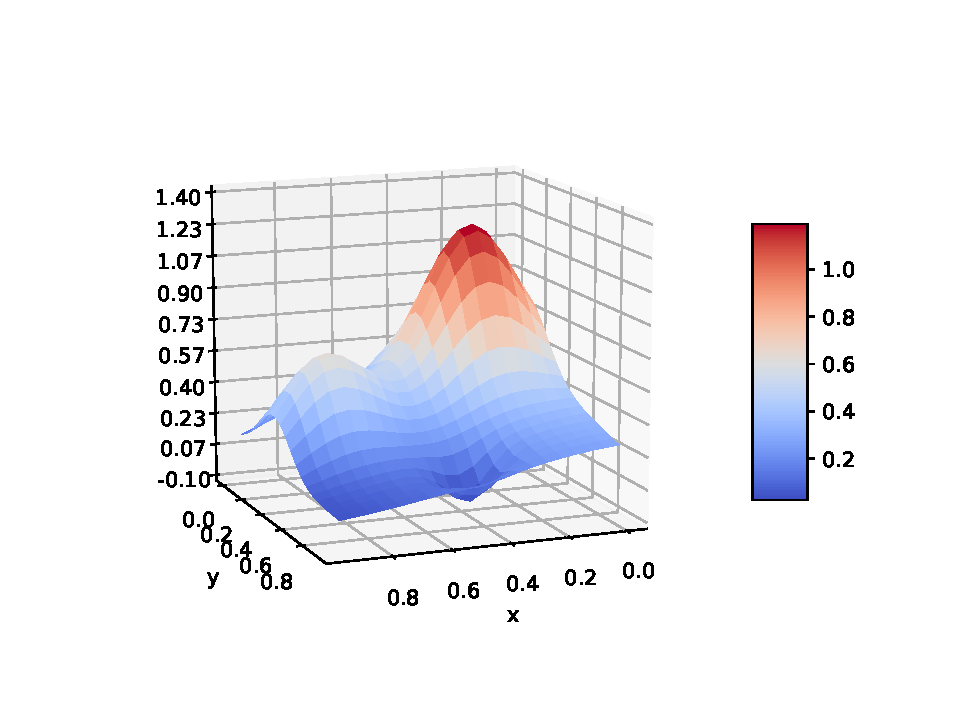
\includegraphics[scale=0.7]{../Results/Part_a/frankeplot.pdf} 
        \caption{\eqref{eq:Frankes} $x,y\in [0,1]$ with grid spacing $0.05$}
        \label{fig:franke}   
\end{figure}  
\subsection{Code implementation}
The regression methods are implemented into a program using Python 2.7, using numpy and Scikit-learn. The code is structured around a program which contains a data class, with methods for different regression procedures, as well as data generation and data reading. The results presented in the following section are produced using their own smaller programs, which draw on the classes from the main program. The class method for Lasso uses the Scikit-learn, while OLS and Ridge do not. Additionally, the k-Fold CV draws on some utility from Scikit-learn, such as dividing folds.

\subsubsection{Initial evaluation of OLS implementation}\label{S:Code_impl_init_ols}
In order to make an initial evaluation implementation of the OLS regression, terrain data is generated using Franke's Function \eqref{eq:Frankes}, with $30 \times 30$ grid points. One data set with no noise, one with noise $\sim N(0,1)$ and one with $\sim N(0,0.3)$. Polynomials of up to fifth order are directly fitted using the entire data set, and the accuracy of the model fittings are recorded in terms of MSE and $R^2$, as well as $95\%$ confidence interval for the regression coefficients. 

\subsubsection{Test of k-Fold Cross Validation implementation}
Following the test of the OLS method, the k-Fold Cross Validation re-sampling method is tested. The aim of this test is to try to establish a suitable number of folds, $k$. A data set using the same parameters as previously, (with noise $\sim N(0,0.3)$) is used. Under increasing model complexity, the data is split up in folds as described in the \hyperref[M:kfold]{methods sections}. For each value of $k$, the average training data MSE is calculated, so that it may be used as a quality measurement. 

\subsubsection{Bias-Variance trade-off}
Upon concluding that $k=10$ is a suitable number of folds, the kFCV method using OLS regression is now applied to $50$ generated data set, similar parameters as previously, with noise $\sim N(0,0.3)$. For each data set, a design matrix is set up, and $k=10$-fold CV is carried out over increasingly complex models with polynomial degrees ranging from 1 to 10. After the $50$ iterations, mean values of the mean MSE (of the kFCV) on test data and training data are calculated. This final mean over the $50$ iterations, are meant to illustrate the bias-variance trade-off, as well as helping in further establishing a suitable complexity for $n \times n$ grids on Franke's Function.

\subsubsection{Ridge and Lasso implementation testing}
Lasso and Ridge regression is in this project tested and evaluated simultaneously. Using a selected complexities and a range of $\lambda=0$ to $1$, Ridge and Lasso regression is carried out with $10$-fold Cross Validation on the same $30 \times 30$ grid as previously. The MSE values for training and test data for the two regression methods are measured and plotted as functions of $\lambda$, in order to discuss their aptness for terrain prediction.
\section{Results}
\subsection{OLS implementation}
Below, MSE and $R^2$ values for the initial evaluation of the OLS is presented in table \ref{table:OLS_mse_r2} for polynomials up to degree five, using the  $30 \times 30$ Franke's Function generated data set with noise $\sim N(0,0.3)$. Similar tables for noise $\sim N(0,1)$ and no noise can be foind in \hyperref[APP_2]{appendix 2}. These tables clearly show that both $R^2$ values and MSE decrease with increased model complexity up to the fifth degree, and that both measurements increase with increased noise.  
%MSE r2 TABLE
\begin{table}[h!]
\begin{center}
\begin{tabular}{lll}
\hline
 Polynomial degree   & $R^2$      & MSE        \\
\hline
 $ 1 $               & $ 0.3521 $ & $ 0.1169 $ \\
 $ 2 $               & $ 0.3947 $ & $ 0.1093 $ \\
 $ 3 $               & $ 0.4519 $ & $ 0.0989 $ \\
 $ 4 $               & $ 0.4904 $ & $ 0.0920 $ \\
 $ 5 $               & $ 0.5032 $ & $ 0.0897 $ \\
\hline
\end{tabular}
\end{center}
\caption{MSE and $R^2$ scores for OLS on  Franke's Function generated responses using a $30\times 30$ grid with noise $\sim N(0,0.3)$ }
\label{table:OLS_mse_r2}
\end{table}

Figure \ref{fig:betas_all} shows the spread of confidence intervals for a 1. order up to 5. order fitting using OLS on the $30 \times 30$ Franke's Function generated grid with noise $\sim N(0,0.3)$. Looking at the figure, it is evident that the magnitude of the largest coefficients increase with increased complexity. Furthermore, $\beta_0$ appears to stay stationary at a small positive magnitude. This also appears to be that case for  $\beta_1$ and $\beta_2$, which corresponds to the response dependency on $x$ and $y$. As the confidence intervals for the coefficients are mostly small relative to the spread of the coefficient's values, a second plot showing the confidence intervals of a fifth order fitting is shown in figure \ref{fig:betas_fifth}. From said figure, it is clear that coefficients with large values have a larger uncertainty. 

%CI of BETA
\begin{figure}[!h]
        \centering 
         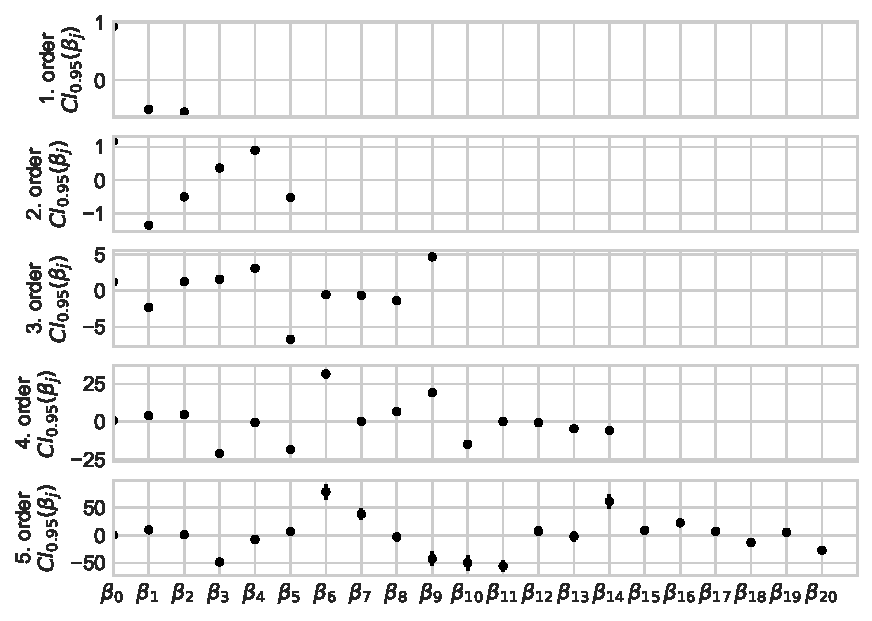
\includegraphics[scale=0.7]{../Results/Part_a/betas_franke_all_noise03.pdf} 
        \caption{$95\%$ confidence intervals for the OLS regression coefficients for polynomials of order one to five, using the Franke's Function generated response on a $30\times 30$ grid}
        \label{fig:betas_all}   
\end{figure}  

%CI of BETA for P=5
\begin{figure}[!h]
        \centering 
         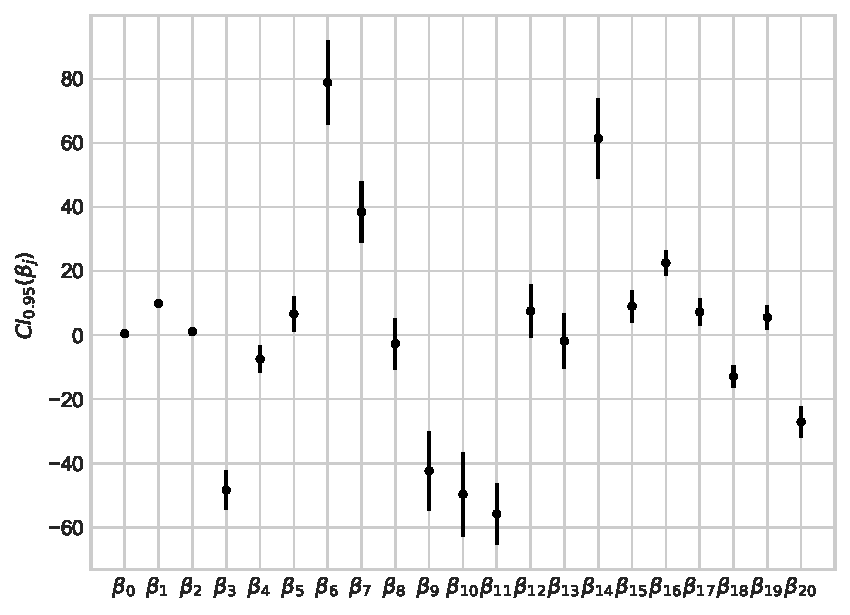
\includegraphics[scale=0.7]{../Results/Part_a/Part_abetas_franke_p5_noise03.pdf} 
        \caption{$95\%$ confidence intervals for the OLS regression coefficients for a fifth order polynomial, using the Franke's Function generated response on a $30\times 30$ grid}
        \label{fig:betas_fifth}   
\end{figure}  

\subsection{Test of k-Fold Cross Validation implementation}
Figure \ref{fig:kfold_kval} shows the average MSE from $k=5,10,20,40$ folds on the same data set. Having already established a decrease in MSE for this type of data set following complexity increase up to fifth order polynomials, the mean MSE values are shown as functions of model complexity in range from $4$ up to $9$, in order to further investigate the complexity-accuracy relationship. It is evident that MSE initially decreases with complexity, before increasing at the sixth order for all values of $k$. In addition, the figure indicates that $k=5$ fold CV yields decreased accuracy in comparison to higher $k$ values, while $k=10,20,$ and $40$ have approximately the same MSE, with a minimum of $\sim 0.89$ at the fifth order of complexity.


\begin{figure}[!h]
        \centering 
         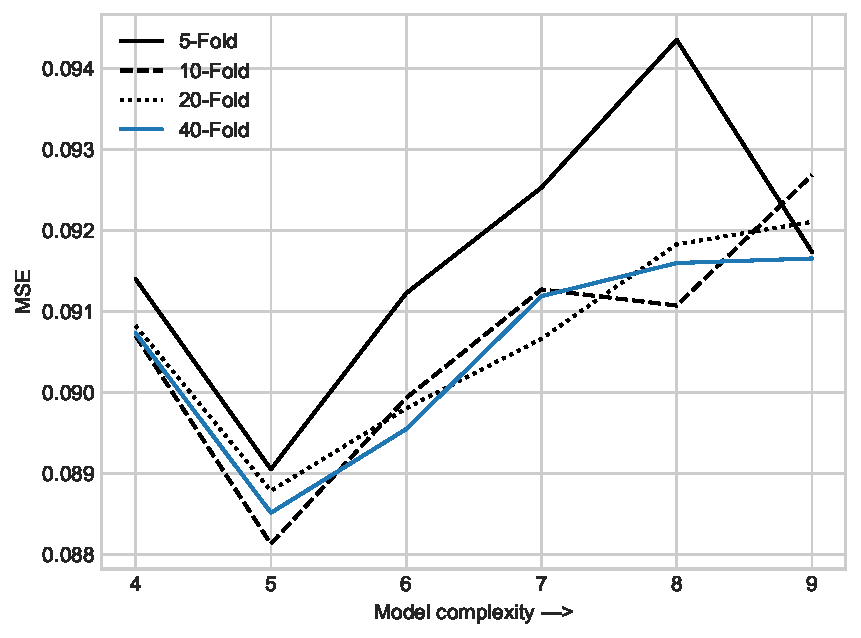
\includegraphics[scale=0.7]{../Results/Part_b/kfold_foldeval.pdf} 
        \caption{Comparison of produced average MSE from training data using OLS with k-Fold CV under increasing model complexity for $k=10,20,20,40$. Data originates from Franke's Function generated response on a $30\times 30$ grid}
        \label{fig:kfold_kval}   
\end{figure}  


\subsection{Bias-Variance}
Figure \ref{fig:bias_var_OLS} shows averaged mean MSE from kFCV using OLS of varying complexity over $50$ data sets. It is evident from the plots, that - when averaged over many data sets - the MSE from training and test data first decrease proportionally, then diverge, with increased complexity.  For complexity corresponding 4th, 5th, 6th and 7th order polynomials, the averaged test MSE appears to be at a minimum $\sim 0.095$. For polynomials of higher order than $7$, the test MSE increases above $\sim 0.095$ towards $1$.


\begin{figure}[!h]
        \centering 
         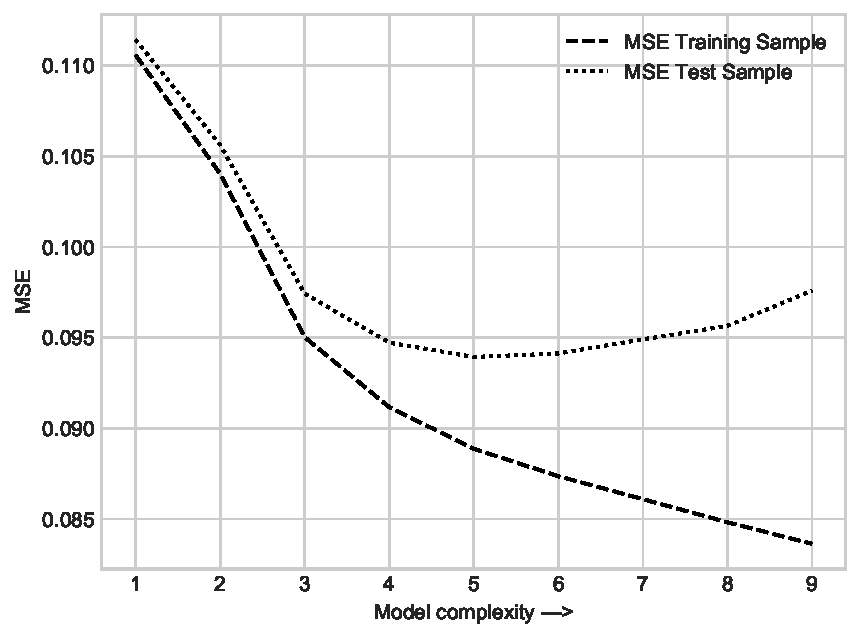
\includegraphics[scale=0.7]{../Results/Part_C/bias_var_50runs.pdf} 
        \caption{Comparison of kFCV ($k=10$) mean MSE using OLS from training and test data of varying complexity, averaged over $50$ data sets generated from Franke's Function on a $30\times 30$ with noise $\sim N(0,0.3)$.}
        \label{fig:bias_var_OLS}   
\end{figure}  



\subsection{Ridge and Lasso}
\ref{fig:ridgelasso_kfold} shows test and training MSE for Ridge and Lasso regression for a number of $\lambda$ values for selected complexities, based on the same data set as in the last kFCV examination. Based on the plot $\lambda \rightarrow 0$ seems to produce the most accurate results for Ridge regression, while the choice of $\lambda$ appears somewhat arbitrary in the for Lasso regression. Additionally, MSE (for both test and training) seems to increase drastically for any values of $\lambda>0$.
\begin{figure}[!h]
        \centering 
         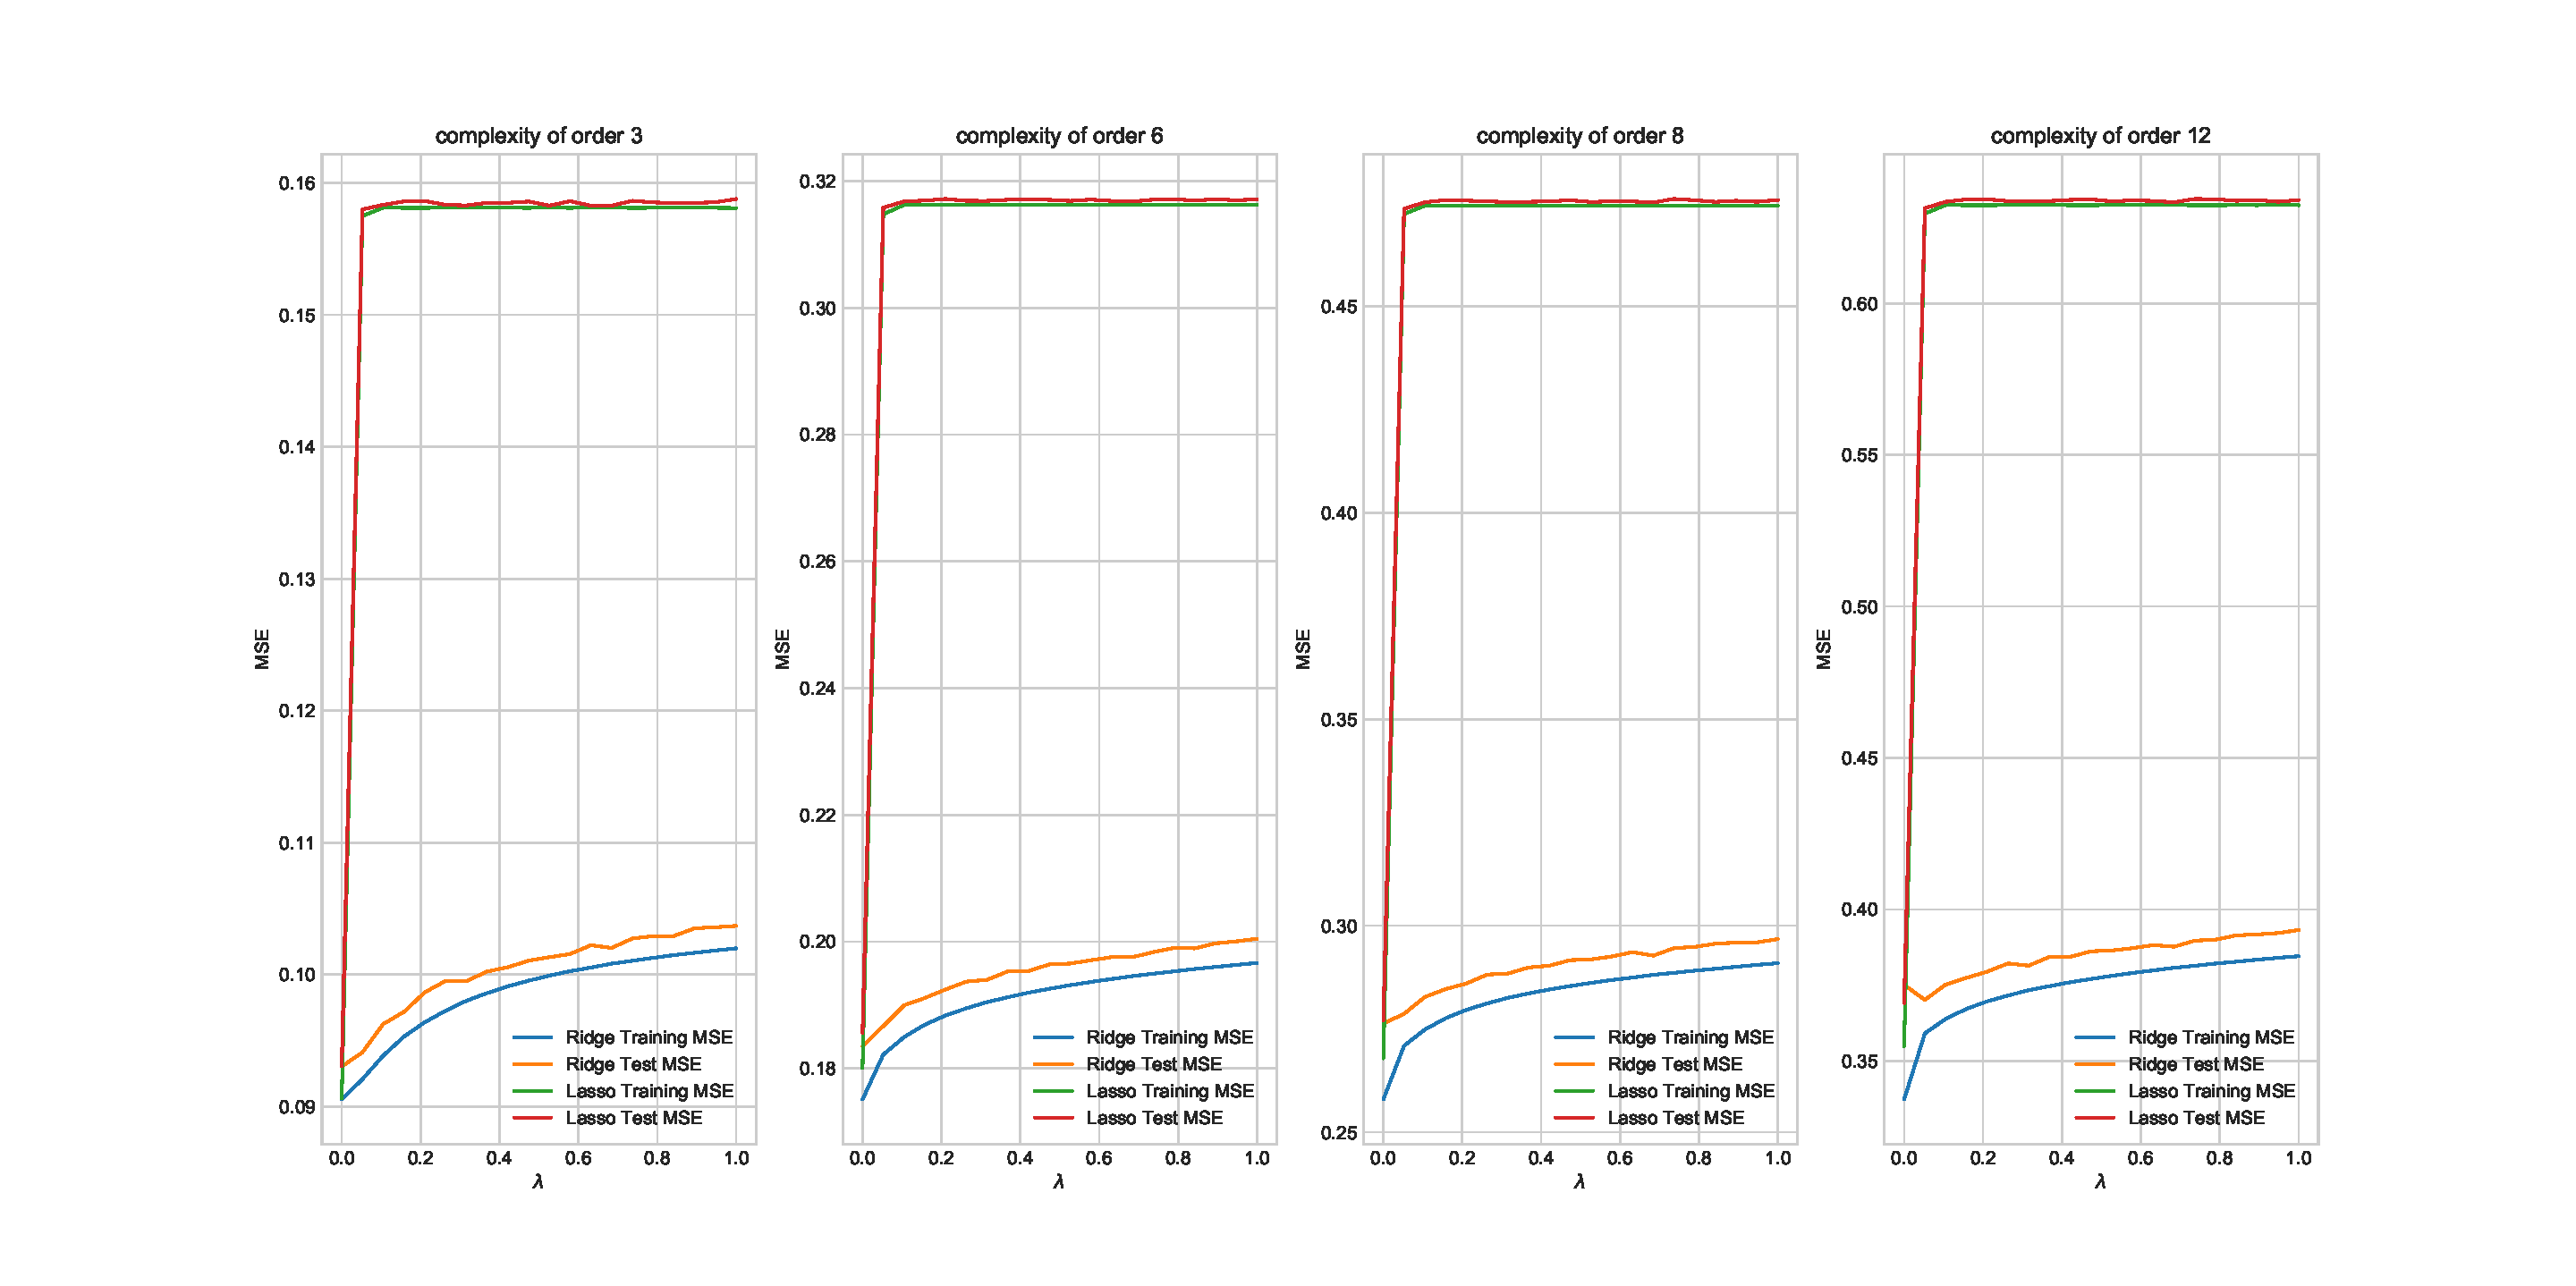
\includegraphics[scale=0.35]{../Results/Part_d/ridgelasso_kfold.pdf} 
        \caption{Test and training MSE for a range of $\lambda \in [0,1]$, for Ridge and Lasso regression using $k=10$ fold CV, over selected complexities}
        \label{fig:ridgelasso_kfold}   
\end{figure}  
\section{Discussion of results}
\subsection{OLS implementation}
As Franke's Function does not describe a planar terrain, the increased $R^2$ score and decreased MSE with increased model complexity  is no surprise.  The small, and approximately stationary values of $\beta_1$ and $\beta_2$  is neither surprising, as \ref{fig:franke} suggests that there are no general drastic changes associated with $x$ and $y$ to the power of one. However, \ref{fig:franke} indicates that values of $x$ and $y$ close to zero should produce a high response. In speculative terms, it is possible that the large positive coefficients are a result of this - especially because they correspond to high powers of the domain variables. On the large(($\pm \sim 20$) confidence intervals observed on those coefficients it is, in the same uncertain terms, possible that perturbation on higher powers of $x$ and $y$ cause large intervals. 

\subsection{k-Fold CV}
The initial decrease in mean MSE follows the trend seen in the OLS implementation testing.  As was observed previously, and again in the kFCV test, a complexity corresponding to a fifth order polynomial appears to be the most accurate, with a minimum mean MSE $\sim 0.89$. This holds true for $k=5,10,20,40$ - albeit $k=5$ exhibits significant inaccuracy relative to the other $k$-values, especially so when complexity further increases. Lower $k$ values mean larger subset for both training and testing, but fever iterations. This may possibly results in less bias, as the training folds become closer to the entirety of the data. Simultaneously, this may also increase variance, although this is not explicitly shown in the results. Tendencies related to the bias-variance trade-off are however present. As increases in $k$ are also more computationally expensive, $k=10$ appears to be a suitable value.

\subsection{Bias-Variance}
Following the trend observed in the initial k-Fold Cross-Validation test, a clear indication of bias-variance trade-off is observed for complex models using OLS regression. Averaging MSE $\sim 0.095$ on 4th-7th order polynomials, the test data MSE then increases towards MSE $\sim 1$ for further increased complexity, while the training MSE continues to decrease. This is highly likely due to the better reproduction of training data at the cost of general validity on other samples from the same main population. The exact optimum polynomial degree is difficult to ascertain, although the simulations points towards a fifth order. Due to the averaging over 50 data sets, this candidate for optimal complexity is somewhat strengthened, but this is at the same time only for the specific $30 \times 30$ grid with noise $\sim N(0,0.3)$. Due to this fact, this project reaches no specific conclusions on optimal polynomial degree. However, if the Franke's Function generated grid is somewhat representative for terrain data, polynomials above the 4th order, and below the 8th order appears to be preferable.

\subsection{Ridge and Lasso}
Surprisingly, $\lambda > 0$ appears to produce the increasingly inaccurate results for both Lasso and Ridge regression on the evaluation data sets. For Lasso, increasing values for $\lambda$ seems to produce especially inaccurate predictions, with a significant, almost step-wise, increase after $\lambda=0$. This may indicate that OLS regression, that is, no shrinkage, is the preferred regression method for the Franke's Function generated data. Going by the description of these procedures in the methods sections however, one would not necessarily be inclined to expect this. This means that there is a distinct possibility that the implementation of the two algorithms is faulty. As this parameter evaluation is only superficial, these results carry no implication beyond indicating that OLS is the preferred regression method when using the programs written for the purpose of this project. It is also worth mentioning that for $\lambda=0$, the Lasso Method produces convergence warnings.


\subsection{Conclusions}



\bibliography{ref}
\bibliographystyle{plain}

\begin{appendices}
\section*{Appendix 1.} \label{APP_1}
Following \citep{HastieTrevor2009TEoS}[p.223]
følg https://stats.stackexchange.com/questions/204115/understanding-bias-variance-tradeoff-derivation

\section*{Appendix 2.} \label{APP_2}
\begin{table}[h!]
\begin{center}
\begin{tabular}{lll}
\hline
 Polynomial degree   & $R^2$      & MSE        \\
\hline
 $ 1 $               & $ 0.7405 $ & $ 0.0176 $ \\
 $ 2 $               & $ 0.8140 $ & $ 0.0126 $ \\
 $ 3 $               & $ 0.9115 $ & $ 0.0060 $ \\
 $ 4 $               & $ 0.9561 $ & $ 0.0030 $ \\
 $ 5 $               & $ 0.9840 $ & $ 0.0011 $ \\
\hline
\end{tabular}
\end{center}
\caption{MSE and $R^2$ scores for OLS on  Franke's Function generated responses using a $30\times 30$ grid without noise}
\label{table:OLS_mse_r2}
\end{table}

\begin{table}[h!]
\begin{center}
\begin{tabular}{lll}
\hline
 Polynomial degree   & $R^2$      & MSE        \\
\hline
 $ 1 $               & $ 0.0865 $ & $ 0.9102 $ \\
 $ 2 $               & $ 0.0999 $ & $ 0.8968 $ \\
 $ 3 $               & $ 0.1099 $ & $ 0.8868 $ \\
 $ 4 $               & $ 0.1145 $ & $ 0.8822 $ \\
 $ 5 $               & $ 0.1285 $ & $ 0.8683 $ \\
\hline
\end{tabular}
\end{center}
\caption{MSE and $R^2$ scores for OLS on  Franke's Function generated responses using a $30\times 30$ grid with noise $\sim N(0,1)$ }
\label{table:OLS_mse_r2}
\end{table}


\end{appendices}

\end{document}